%!TEX encoding = UTF-8 Unicode
\section{実装評価}
\subsection{緒言}
本章では,前章で実装した提案手法を用いて,評価を行った結果について説明する.はじめに,評価環境と評価条件について説明する.その後,提案手法の実装において考慮すべき実行時のオーバヘッドの測定結果について,定量的に説明する.\par

\subsection{動作確認}


\subsection{評価環境}
はじめに,評価環境について説明する.ウェブインタフェースをウェブ機能とスケジューラ抽象化機能に分離したことによって両者の連携時のオーバヘッドの発生が懸念されるため,その影響を定量的に評価する.本実装においては,OODがシェルを介してPSI/JのPythonスクリプトを実行するため,そのオーバヘッドによる影響を評価する.\par
評価には,Selenium\cite{cite6}と呼ばれるウェブブラウザの自動制御ライブラリを用いる.機能の分離前と分離後を比較したいため,OODがNQSVに対応していないことから評価環境として疑似AOBAクラスタを用いることはできない.そこで,実験用に用意したSlurmクラスタを用いて機能分離に伴うオーバヘッドの評価を行う.Slurmクラスタのマスターノードとワーカーノードの詳細情報を表\ref{masternode},表\ref{workernode}に示す.\par

\begin{table}[b]
    \begin{minipage}[c]{0.5\hsize}
        \centering
        \begin{tabular}{lr}
            \multicolumn{2}{c}{マスターノード} \\ \hline
            CPU    & Intel Xeon W-2102  \\
            メモリ容量  & 512GB              \\
            コア数    & 4                  \\
            OS     & Ubuntu 22.04.2 LST \\
            RAM    & 16GB              
        \end{tabular}%
        \caption{マスターノード}
        \label{masternode}
    \end{minipage}%
    \begin{minipage}[c]{0.5\hsize}
        \centering
        \begin{tabular}{lr}
            \multicolumn{2}{c}{ワーカーノード} \\ \hline
            CPU    & Intel Xeon E-2378  \\
            メモリ容量  & 512GB              \\
            コア数    & 8                  \\
            OS     & Ubuntu 22.04.2 LST \\
            RAM    & 64GB              
        \end{tabular}%
        \caption{ワーカーノード}
        \label{workernode}
    \end{minipage}
\end{table}

評価環境を図\ref{evaluation_environment}に示す.ローカルホストからOODホストサーバのウェブブラウザにアクセスして,ユーザ名とパスワードを用いてログインする.ダッシュボード画面からJob Composer画面に移動し,New Jobボタンを押下する.選択肢の中からFrom Specified Pathを選択してジョブが配置されたディレクトリ,ジョブスクリプトのファイル名,実行するクラスタ名を選択して,ジョブの作成と投入を行う.投入したジョブの状態はsqueueコマンドにより確認し,コマンドの出力結果によってジョブの実行完了を確認する.New Jobボタンを押下した時刻から,そのジョブの実行を完了した時刻までを計測し,ジョブのターンアラウンドタイムとする.OODは過去に投入したジョブの履歴が残るという仕様があるため,ターンアラウンドタイムの計測終了後にJob Composer画面のdeleteボタンからジョブの履歴を削除する.また,本研究では,機能分離後のターンアラウンドタイムと機能分離前のターンアラウンドタイムの差分をオーバヘッドと定義する.\par

\begin{figure}[tb]
    \centering
    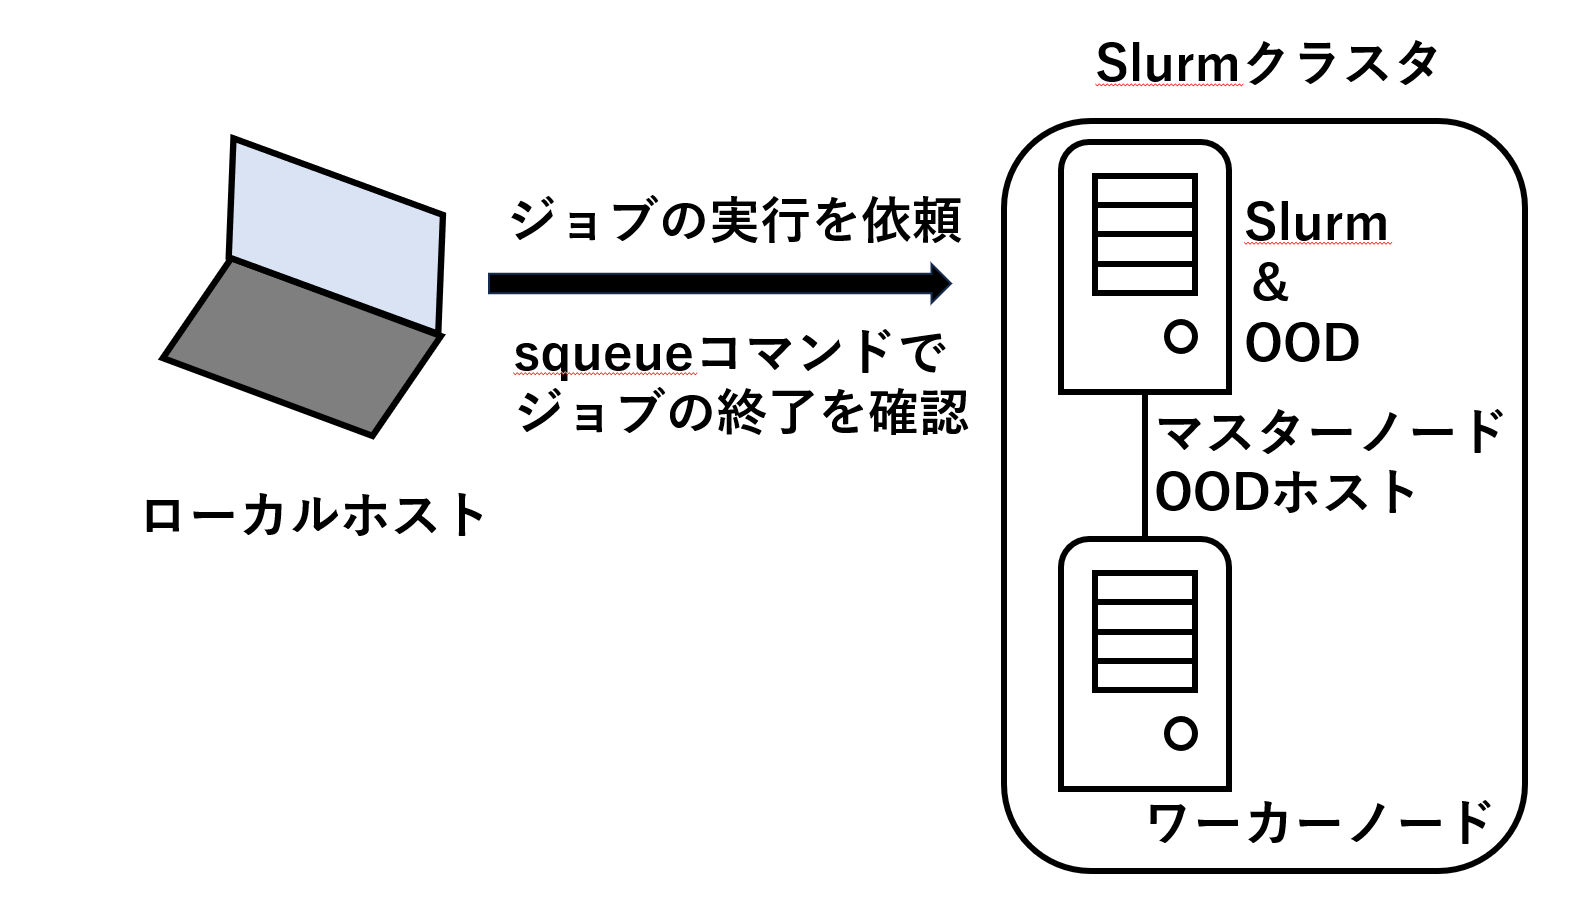
\includegraphics[width=120mm]{./fig/evaluation_environment.png}
    \caption{評価環境}
    \label{evaluation_environment}
\end{figure}

\subsection{評価条件}
評価条件について説明する.はじめに,単一ジョブを機能分離前後で50回ずつ投入したときのターンアラウンドタイムを比較する.続いて,ジョブの投入を1~10回連続で行い,そのターンアラウンドタイムを計測してPSI/Jを経由する場合と経由しない場合を比較する.ターンアラウンドタイムは1~10回の連続投入でそれぞれ50回ずつ計測る.その後,ジョブを1~100回連続投入した際のターンアラウンドタイムの比較を行う.ジョブの連続投入数は1回から開始して10回ずつ増やしていき,ジョブ数を大きくした場合の結果を得る.\par

\subsection{実行時オーバヘッドの評価}
はじめに,単一ジョブを機能分離前後で50回ずつ投入したときのターンアラウンドタイムの箱ひげ図を図\ref{boxplot}に示す.左側のデータセットが機能分離前,右側のデータセットが機能分離後を示し,縦軸はターンアラウンドタイムを示す.外れ値を除外すると両データセットには有意差が見られる.機能分離前のターンアラウンドタイムの平均値は17.67秒であり,機能分離後のターンアラウンドタイムの平均値は20.53秒である.結果から,単一ジョブ実行時のオーバヘッドは20.53-17.67=2.86秒と算出される.オーバヘッドは機能分離前のターンアラウンドタイムの16\%程度であることがわかる.\par

\begin{figure}[tb]
    \centering
    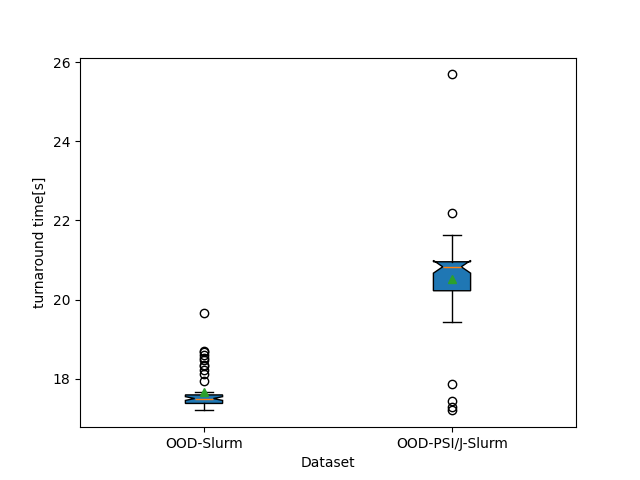
\includegraphics[width=120mm]{./fig/boxplot.png}
    \caption{機能分離前後での単一ジョブ実行によるターンアラウンドタイム}
    \label{boxplot}
\end{figure}

続いて,1~10回のジョブの連続投入により得られた評価結果を図\ref{fig8}および図\ref{fig9}に示す.図\ref{fig8}では機能分離前後でのターンアラウンドタイムをエラーバー付きで比較する.横軸は連続して投入したジョブの数,縦軸はターンアラウンドタイムを示す.図\ref{fig9}は機能分離によるオーバヘッドを示す.横軸は連続して投入したジョブの数,縦軸はジョブ実行時のオーバヘッドを示す.図\ref{fig8}から機能分離後の方がターンアラウンドタイムが大きいことがわかり,機能分離前後での結果に有意な差があることがわかる.機能の分離にかかわらず,どちらの場合も連続投入したジョブの数に線形比例して増加していることがわかる.また図\ref{fig9}から,ジョブの連続投入回数が増加するほど,機能分離によるオーバヘッドも線形増加していることがわかる.したがって,図\ref{fig8},図\ref{fig9}から1ジョブあたりのオーバヘッドの大きさは変化していないことがわかる.\par

\begin{figure}[tb]
    \centering
    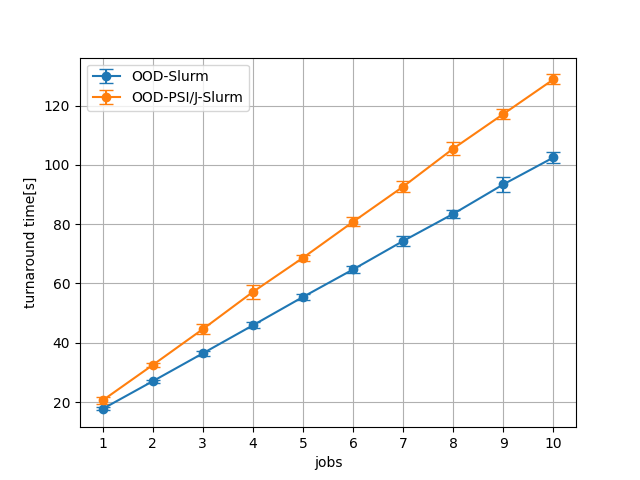
\includegraphics[width=120mm]{./fig/1-10jobs.png}
    \caption{機能分離前後でのターンアラウンドタイムの比較}
    \label{fig8}
\end{figure}
  
\begin{figure}[tb]
    \centering
    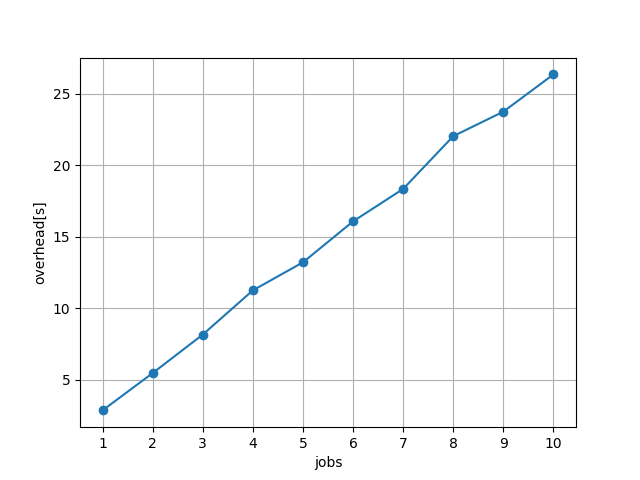
\includegraphics[width=120mm]{./fig/1-10_overhead.png}
    \caption{機能分離によるオーバヘッド}
    \label{fig9}
\end{figure}


ジョブを1~100回連続投入した際の機能分離前後のターンアラウンドタイムの比較を図\ref{fig10}に示す.横軸は連続して投入したジョブの数,縦軸はターンアラウンドタイムを示す.1~10回の連続投入の場合と同じく,PSI/Jを経由した場合の方がわずかにターンアラウンドタイムが大きくなっており,連続投入するジョブ数を大きくしても極端にオーバヘッドに差が出ることはないということがわかった.\par
様々なジョブの連続投入回数でのターンアラウンドタイムの結果から,ジョブ実行時のオーバヘッドを測定した.その結果から,ジョブの連続投入回数に依らず,PSI/Jを経由した場合のオーバヘッドは,PSI/Jを経由しない場合のターンアラウンドタイムの5%以内に収まり,提案手法によって生じるオーバヘッドは十分無視できるといえる.\par

\begin{figure}[tb]
    \centering
    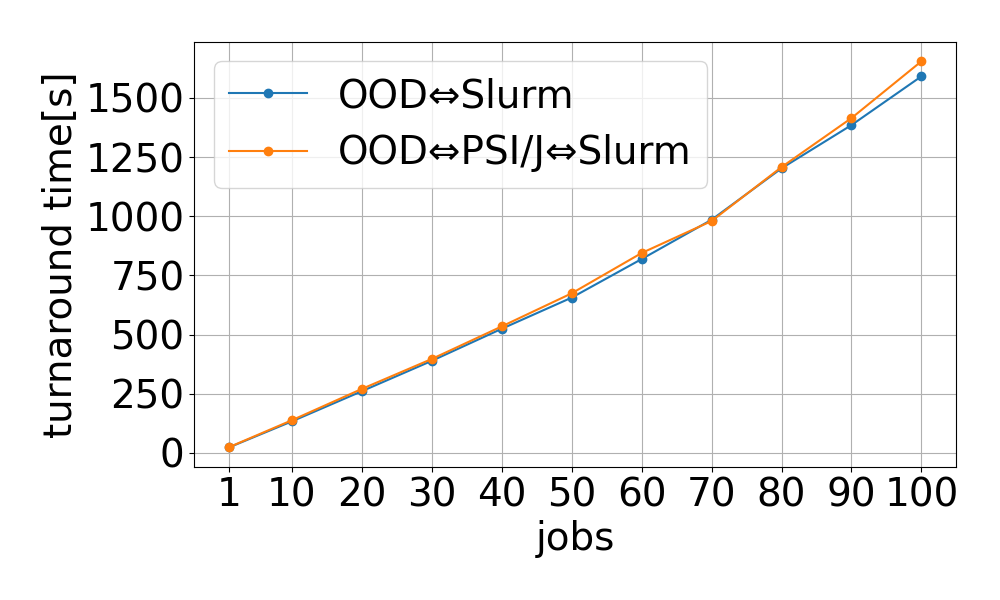
\includegraphics[width=120mm]{./fig/100jobs.png}
    \caption{ジョブ数を増加した際のターンアラウンドタイムの比較}
    \label{fig10}
\end{figure}

\subsection{結言}
本章では,実際にジョブの投入を行った際の提案手法の実装の評価結果を示した.はじめに,評価を行う環境について説明した.その後,機能の分離前後で生じるオーバヘッドを測定する際の評価条件について説明した.これらの評価環境と評価条件により得られた評価結果により,提案手法により生じるオーバヘッドは充分小さいため実用上は問題ないということを示した.\par